\documentclass[tikz,border=10pt]{standalone}
\begin{document}
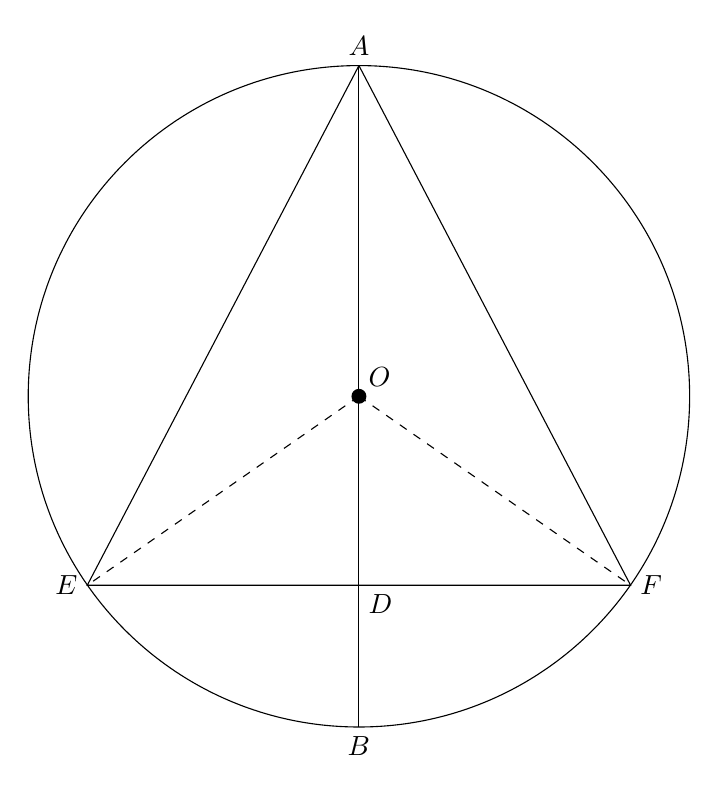
\begin{tikzpicture}[scale=3]
  \coordinate (O) at (0,0);
  \coordinate (A) at (0,1.4);
  \coordinate (B) at (0,-1.4);
  \coordinate (E) at (-1.15,-0.8);
  \coordinate (F) at (1.15,-0.8);
  \coordinate (D) at (0,-0.8);

  \draw (O) circle (1.4);
  \draw (A) -- (E) -- (F) -- (A);
  \draw (A) -- (B);
  \draw[dashed] (O) -- (E);
  \draw[dashed] (O) -- (F);

  \fill (O) circle (0.9pt);

  \node[above] at (A) {$A$};
  \node[below] at (B) {$B$};
  \node[left] at (E) {$E$};
  \node[right] at (F) {$F$};
  \node[below right] at (D) {$D$};
  \node[above right] at (O) {$O$};
\end{tikzpicture}
\end{document}
